\documentclass[12pt,a4paper]{article}
\usepackage[utf8]{inputenc}
\usepackage[italian]{babel}
\usepackage{geometry}
\usepackage{graphicx}
\usepackage{hyperref}
\usepackage{fancyhdr}
\usepackage{titlesec}
\usepackage{enumitem}
\usepackage{xcolor}
\usepackage{listings}
\usepackage{tcolorbox}
\usepackage{amsmath}
\usepackage{booktabs}

% Configurazione della pagina
\geometry{margin=2.5cm}
\setlength{\headheight}{15pt} % Fix for fancyhdr warning
\pagestyle{fancy}
\fancyhf{}
\rhead{BookRecommender - Manuale Utente}
\lhead{Versione 1.0}
\cfoot{\thepage}

% Configurazione dei colori
\definecolor{primaryblue}{RGB}{41, 128, 185}
\definecolor{darkgray}{RGB}{52, 73, 94}
\definecolor{lightgray}{RGB}{236, 240, 241}

% Configurazione delle sezioni
\titleformat{\section}{\Large\bfseries\color{primaryblue}}{\thesection}{1em}{}
\titleformat{\subsection}{\large\bfseries\color{darkgray}}{\thesubsection}{1em}{}

% Configurazione dei listing per il codice
\lstset{
    backgroundcolor=\color{lightgray},
    basicstyle=\ttfamily\footnotesize,
    breaklines=true,
    captionpos=b,
    commentstyle=\color{darkgray},
    frame=single,
    keywordstyle=\color{primaryblue},
    language=Java,
    numbers=left,
    numberstyle=\tiny\color{darkgray},
    showstringspaces=false,
    stringstyle=\color{red},
    tabsize=2
}

% Box per note importanti
\newtcolorbox{infobox}{
    colback=lightgray,
    colframe=primaryblue,
    boxrule=1pt,
    arc=3pt,
    left=6pt,
    right=6pt,
    top=6pt,
    bottom=6pt
}

\begin{document}

% Pagina del titolo
\begin{titlepage}
    \centering
    \vspace*{2cm}
    
    {\Huge\bfseries\color{primaryblue} BookRecommender}
    
    \vspace{1cm}
    
    {\Large Sistema di Raccomandazione Libri}
    
    \vspace{2cm}
    
    {\LARGE\bfseries Manuale Utente}
    
    \vspace{1cm}
    
    {\large Versione 1.0}
    
    \vspace{3cm}
    
\includegraphics[width=0.3\textwidth]{img/LogoDoc.png}
    
    \vfill
    
    {\large Data: \today}
    
    \vspace{1cm}
    
    {\large Autore:
                    \\Babini Ariele
                    \\Bottaro Federico}
    
\end{titlepage}

% Indice
\tableofcontents
\newpage

% Introduzione
\section{Introduzione}

BookRecommender è un sistema avanzato di raccomandazione libri sviluppato in Java utilizzando Maven come strumento di gestione delle dipendenze. Il sistema implementa un'architettura client-server che permette agli utenti di ricevere raccomandazioni personalizzate basate sui propri gusti letterari e comportamenti di lettura.

\subsection{Caratteristiche principali}

\begin{itemize}
    \item Sistema di raccomandazione basato su algoritmi di machine learning
    \item Interfaccia client intuitiva e user-friendly
    \item Architettura scalabile client-server
    \item Gestione completa del catalogo libri
    \item Profili utente personalizzabili
    \item Sistema di valutazione e recensioni
\end{itemize}

\subsection{Architettura del sistema}

Il sistema BookRecommender è composto da due componenti principali:

\begin{description}[style=multiline, labelwidth=1.8cm, leftmargin=2.2cm]
    \item[Server] Gestisce la logica di business, il database dei libri e gli algoritmi di
    raccomandazione
    \item[Client] Fornisce l’interfaccia utente per interagire con il sistema
\end{description}

\section{Requisiti di sistema}

Prima di procedere con l'installazione, assicurarsi che il sistema soddisfi i seguenti requisiti:

\subsection{Requisiti hardware}
\begin{itemize}
    \item Processore: Intel Core i3 o equivalente
    \item RAM: Minimo 4 GB, raccomandati 8 GB
    \item Spazio disco: Almeno 1 GB di spazio libero
    \item Connessione di rete per la comunicazione client-server
\end{itemize}

\subsection{Requisiti software}
\begin{itemize}
    \item Java Runtime Environment (JRE) 11 o superiore
    \item Apache Maven 3.6.0 o superiore
    \item Sistema operativo: Windows 11, macOS 10.14 o superiori
\end{itemize}

\begin{infobox}
\textbf{Nota importante:} Verificare che la variabile d'ambiente JAVA\_HOME sia configurata correttamente prima di procedere con l'installazione.
\end{infobox}

\section{Installazione}

\subsection{Installazione del server}

\begin{enumerate}
    \item Scaricare il pacchetto BookRecommender dal repository
    \item Estrarre i file in una directory dedicata
    \item Aprire un terminale nella directory del progetto
    \item Eseguire il comando per compilare il server:
    
    \begin{lstlisting}[language=bash]
mvn clean compile -pl server
    \end{lstlisting}
    
    \item Avviare il server con:
    
    \begin{lstlisting}[language=bash]
mvn exec:java -pl server -Dexec.mainClass="com.bookrecommender.server.ServerMain"
    \end{lstlisting}
\end{enumerate}

\subsection{Installazione del client}

\begin{enumerate}
    \item Nella stessa directory del progetto, compilare il client:
    
    \begin{lstlisting}[language=bash]
mvn clean compile -pl client
    \end{lstlisting}
    
    \item Avviare l'applicazione client:
    
    \begin{lstlisting}[language=bash]
mvn exec:java -pl client -Dexec.mainClass="com.bookrecommender.client.ClientMain"
    \end{lstlisting}
\end{enumerate}

\section{Configurazione}

\subsection{Configurazione del server}

\begin{verbatim}
# Configurazione porta server
server.port=8080

# Configurazione database
db.url=jdbc:h2:mem:bookrecommender
db.username=sa
db.password=

# Configurazione algoritmi di raccomandazione
recommendation.algorithm=collaborative_filtering
recommendation.max_results=10
recommendation.max_results=10
\end{verbatim}

\subsection{Configurazione del client}

\begin{verbatim}
# Configurazione connessione server
server.host=localhost
server.port=8080

# Configurazione interfaccia
ui.theme=default
ui.language=it
\end{verbatim}
\begin{lstlisting}
ui.language=it
\end{lstlisting}

\section{Guida all'uso}

\subsection{Primo avvio}

\begin{enumerate}
    \item Avviare prima il server, poi il client
    \item All'avvio del client, verrà visualizzata la home page dell'applicazione, dalla quale sarà possibile consultare i libri ed effettuare delle ricerche
    \item Nella schermata sarà visibile in basso a sinistra l'icona dell'account dalla quale si potrà effettuare il login o registrarsi
    \item Compilare i campi richiesti per la registrazione:
    \begin{itemize}
        \item Nome
        \item Cognome
        \item Codice Fiscale
        \item Email
        \item Username
        \item Password
    \end{itemize}
    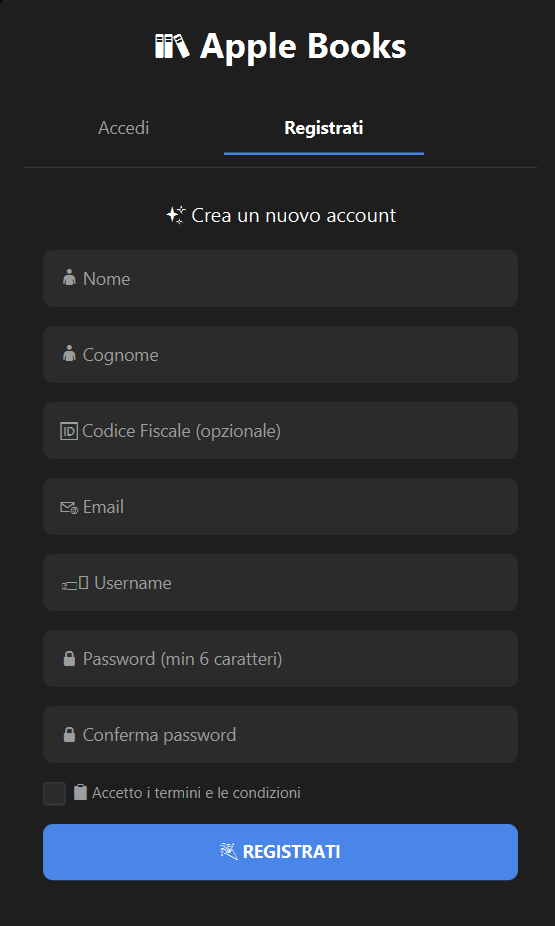
\includegraphics[width=0.3\textwidth]{img/registrati.PNG}
\end{enumerate}

\subsection{Avvi successivi}

Una volta effettuata la prima registrazione si potrà accedere attraverso l'interfaccia di Login inserendo semplicemente mail e password del proprio account.
\\
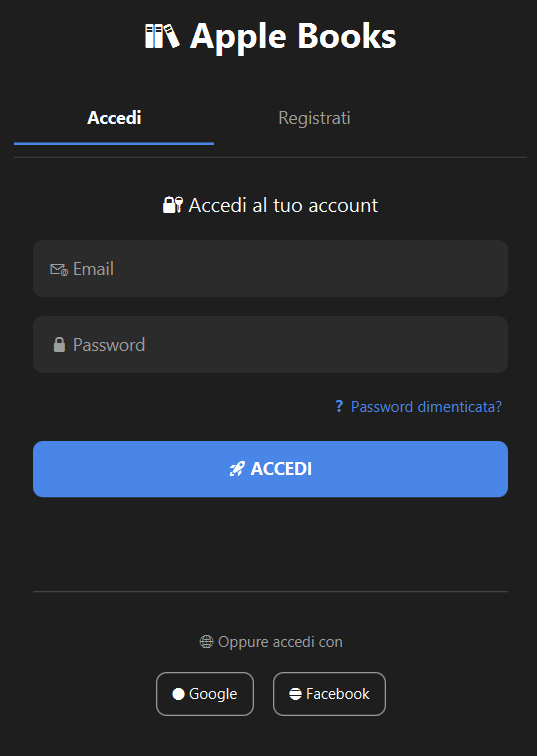
\includegraphics[width=0.3\textwidth]{img/accedi.PNG}
\\
La possibilità di effettuare Login automatico attraverso l'utilizzo di account google verrà implementata successivamente.

\subsection{Interfaccia principale}

L'interfaccia principale del client è divisa in diverse sezioni:

\begin{description}[style=multiline, labelwidth=4cm, leftmargin=4.4cm]
    \item[Menu principale] Accesso alle funzionalità principali
    \item[Catalogo libri] Visualizzazione e ricerca dei libri disponibili
    \item[Raccomandazioni] Libri consigliati basati sul profilo utente
    \item[Profilo utente] Gestione delle preferenze e dello storico
    \item[Biblioteca personale] Libri salvati e letti dall'utente
\end{description}
\textbf{N.B.}
In base al tipo di utente, registrato o utente occasionale, si possono utilizzare diverse funzionalità.
\begin{description}
    \item[Utente non registrato]:
    \begin{itemize}
        \item Ricerca Libri
        \item Visualizzazione valutazioni
        \item Visualizzazione suggerimenti
    \end{itemize}
    \item[Utente registrato]:
    \begin{itemize}
        \item Ricerca Libri
        \item Visualizzazione valutazioni
        \item Visualizzazione suggerimenti
        \item Creazione e gestione di librerie personali per salvare i libri
        \item Inserimento di valutazioni
        \item Inserimento di suggerimenti
    \end{itemize}
\end{description}

\subsection{Ricerca e filtri}

Per trovare libri specifici:

\begin{enumerate}
    \item Utilizzare la barra di ricerca in alto
    \item Applicare filtri per:
    \begin{itemize}
        \item Genere letterario
        \item Autore
        \item Anno di pubblicazione
        \item Valutazione media
    \end{itemize}
    \item Ordinare i risultati per rilevanza, data o valutazione
    \item Utilizzare la voce (Ricerca avanzata) nel menu per effettuare ricerche per:
    \begin{itemize}
        \item Autore
        \item Titolo
        \item Autore e Anno
    \end{itemize}
\end{enumerate}
\textbf{N.B.}
La Ricerca Avanzata restitusice tutti i libri che rispettano i parametri inseriti. (Es. Se nella ricerca per autore viene inserita anche una sola lettera verrano visualizzati tutti i libri il cui autore contiene quella lettera nel nome)

\subsection{Sistema di raccomandazione}

Il sistema offre raccomandazioni basate su:

\begin{itemize}
    \item Trending topics e nuove uscite
    \item Libri con il maggior numero di valutazioni
\end{itemize}

\begin{infobox}
\textbf{Suggerimento:} Per ottenere raccomandazioni più precise, valutare regolarmente i libri letti e aggiornare le preferenze nel profilo.
\end{infobox}

\section{Funzionalità avanzate}

\subsection{Gestione delle librerie}

Gli utenti possono creare librerie personalizzate che permettono di salvare i libri come meglio si preferisce.
\\Le librerie possono essere modificate quando si vuole, permettendo di inserire e rimuovere libri.
\\
\\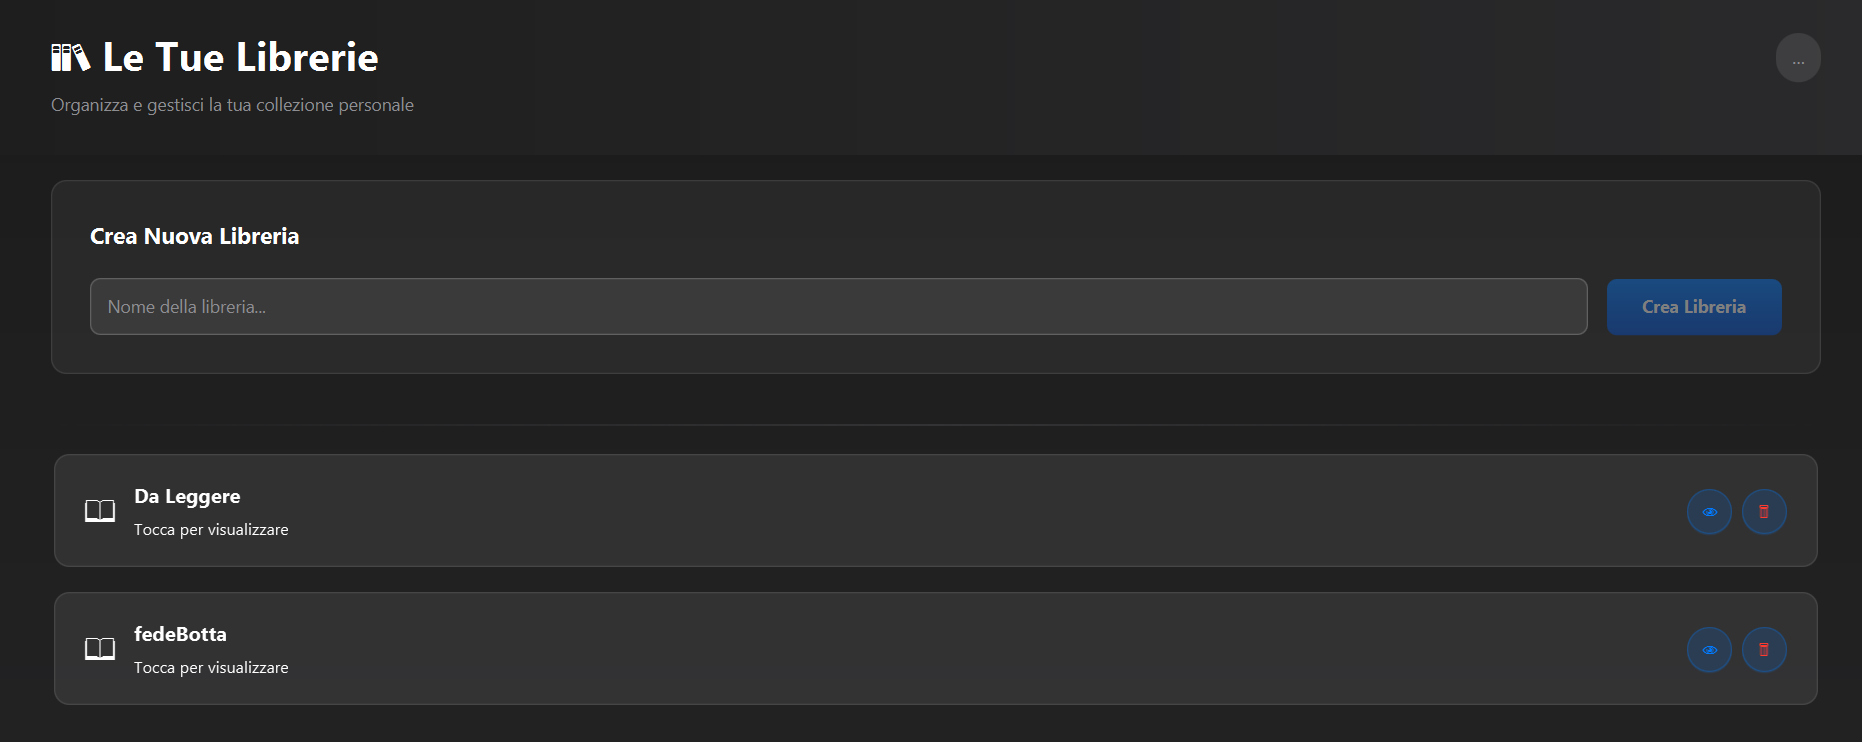
\includegraphics[width=0.8\textwidth]{img/librerie}
\\
\\I libri possono essere inseriti nelle proprie librerie dalla loro interfaccia semplicemente premendo l'apposito tasto "Aggiungi a libreria".
\\
\\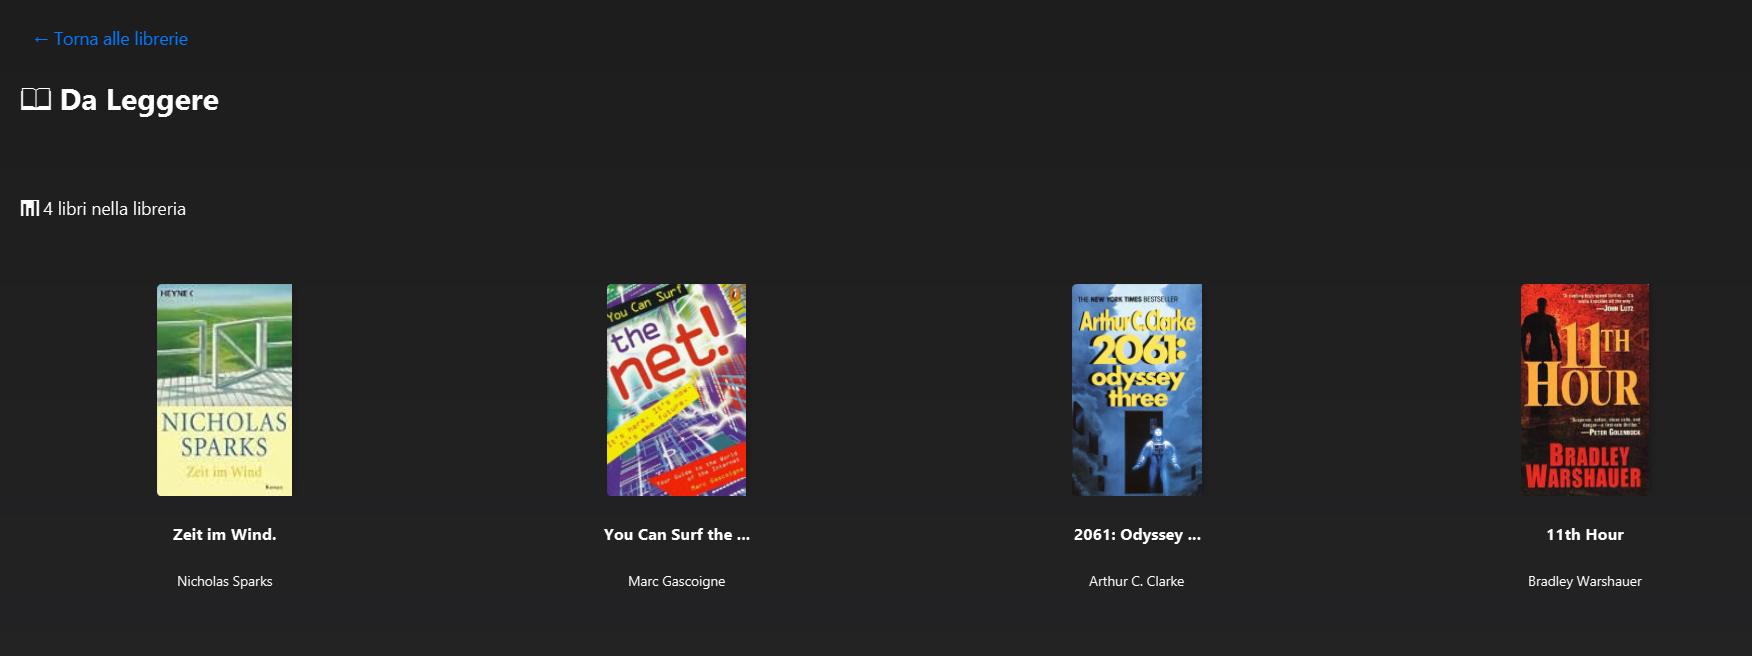
\includegraphics[width=0.8\textwidth]{img/SpecLibreria}
\\
\\
\subsection{Sistema di valutazione}

\begin{itemize}
    \item Valutazione con stelle (1-5)
    \item Recensioni testuali
\end{itemize}
\\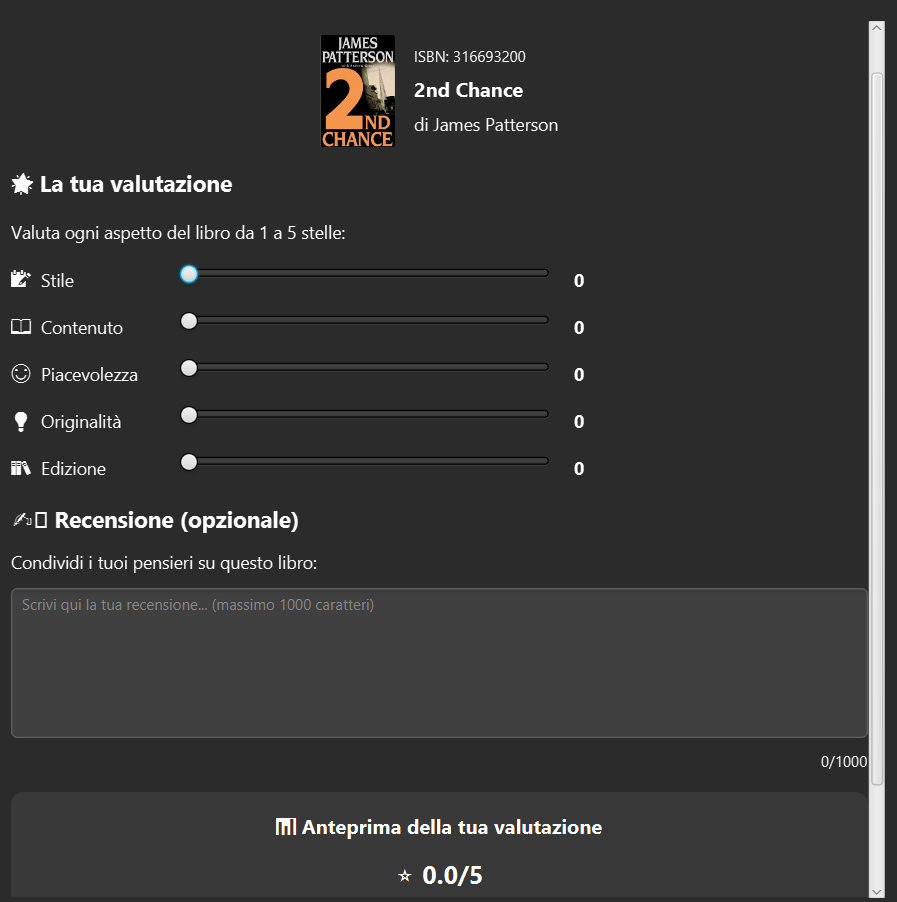
\includegraphics[width=0.8\textwidth]{img/valutazione}

\subsection{Inserimento suggerimenti}

Una delle funzionalità avanzate riservate agli utenti registrati è quella che permette di inserire dei suggerimenti per dei libri (max. 3).
\\L'unico condizione per poter inserire suggerimenti per un libro è quella che quest'ultimo deve trovarsi in una libreria e,
ovviamente, la medesima cosa vale anche per i libro che si vogliono inserire come suggerimenti.
\\Per poter inserire un suggerimento basta selezionare il libro in questione e cliccare sul bottone "Consiglia libri".
\\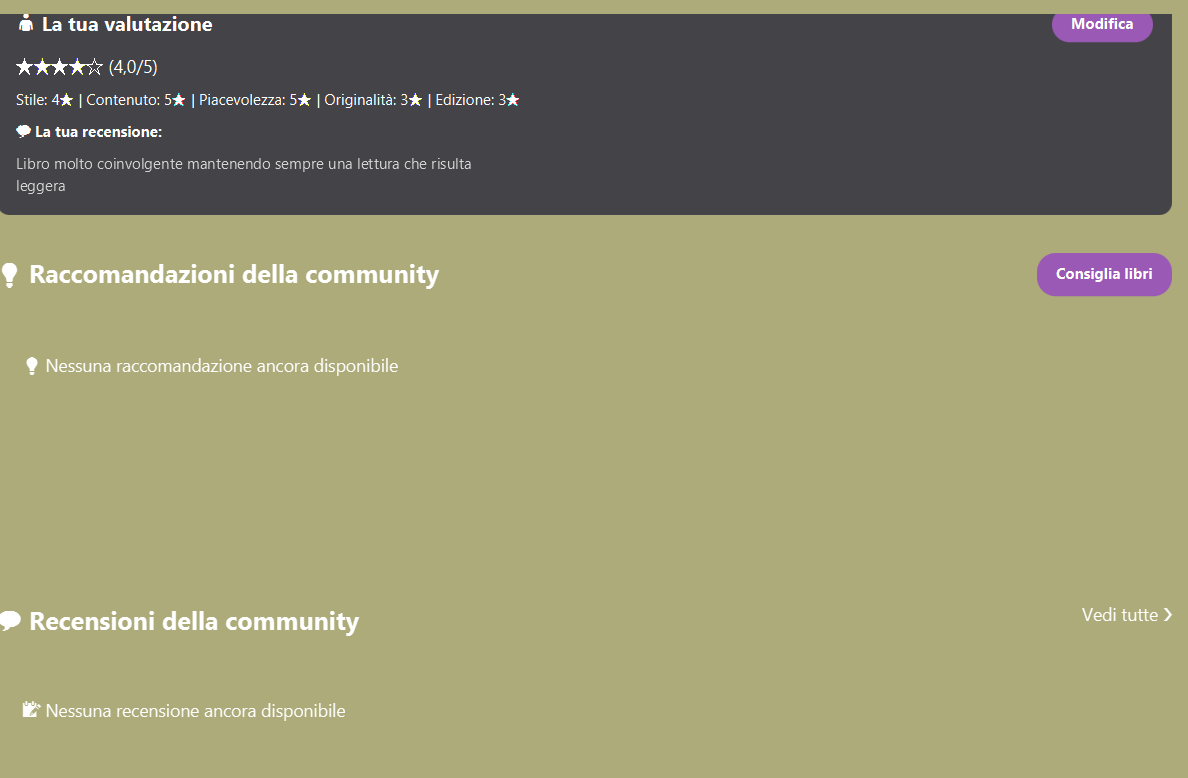
\includegraphics[width=0.8\textwidth]{img/suggerimenti}
\\Una volta cliccato si aprirà un pop-up dal quale sarà possibile selezionare i 3 libri che si vogliono suggerire.
\\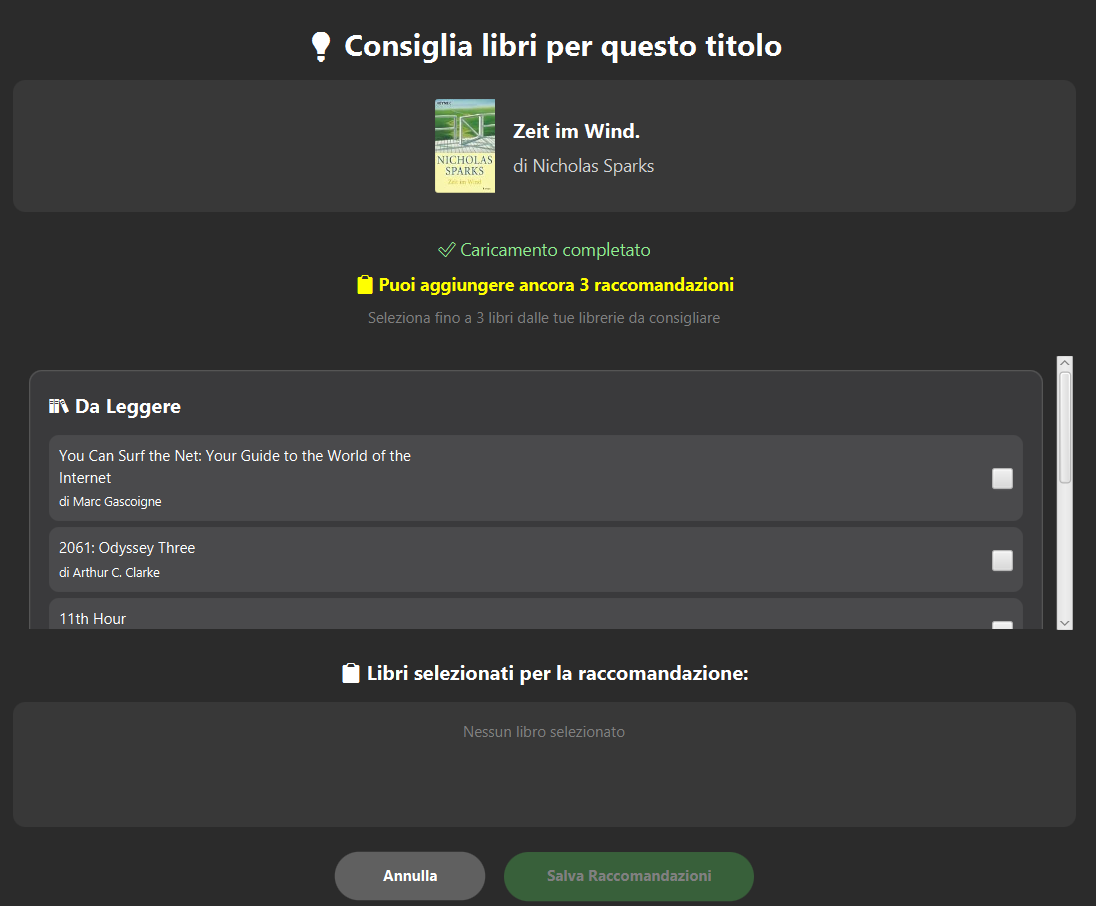
\includegraphics[width=0.8\textwidth]{img/interfacciaSugg}
\\Ovviamente 3 rappresenta il limite massimo, si può aggiungere anche un numero inferiori di libri e, soprattutto, i suggerimenti possono essere modificati quando si vuole eliminando un libro e cambiandolo.
\\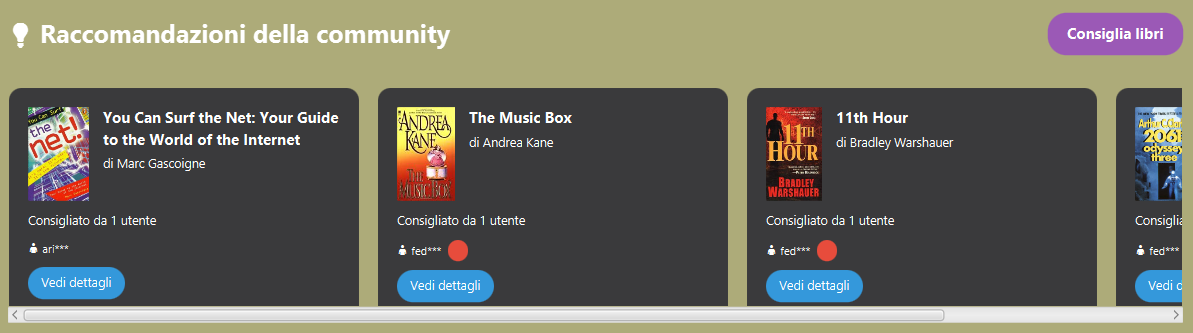
\includegraphics[width=0.8\textwidth]{img/listaSugg}

\subsection{Statistiche personali}

All'interno del pop-up dedicato alla gestione dell'account sono visibili delle statisce personali.

\\Statistiche dettagliate:

\begin{itemize}
    \item Numero di libri presenti nelle librerie
    \item Numero di libri recensiti
    \item Numero di libri suggeriti
\end{itemize}

\section{Troubleshooting}

\subsection{Problemi comuni}

\begin{description}
    \item[Il server non si avvia]
    \item
    \begin{itemize}
        \item Verificare che la porta 8080 non sia occupata
        \item Controllare i log nella directory \texttt{logs/}
        \item Assicurarsi che Java sia installato correttamente
    \end{itemize}
    
    \item[Il client non si connette al server]
    \item
    \begin{itemize}
        \item Verificare che il server sia in esecuzione
        \item Controllare le impostazioni di rete
        \item Verificare la configurazione in \texttt{client.properties}
    \end{itemize}
    
    \item[Le raccomandazioni non sono accurate]
    \item
    \begin{itemize}
        \item Valutare più libri per migliorare l'algoritmo
        \item Aggiornare le preferenze nel profilo
        \item Verificare la configurazione degli algoritmi
    \end{itemize}
\end{description}

\subsection{Log e debugging}

I file di log si trovano nella directory \texttt{logs/}:

\begin{itemize}
    \item \texttt{server.log} - Log del server
    \item \texttt{client.log} - Log del client
    \item \texttt{recommendation.log} - Log degli algoritmi di raccomandazione
\end{itemize}

Per abilitare il debug dettagliato, modificare il file \texttt{logback.xml}:

\begin{lstlisting}[language=xml]
<logger name="com.bookrecommender" level="DEBUG"/>
\end{lstlisting}
\
\
\
\section{API e integrazione}

\subsection{API REST del server}

Il server espone le seguenti API:

\begin{table}[h]
\centering
\begin{tabular}{@{}lll@{}}
\toprule
Endpoint & Metodo & Descrizione \\ \midrule
/api/books & GET & Elenco libri \\
/api/books/\{id\} & GET & Dettagli libro \\
/api/recommendations & GET & Raccomandazioni utente \\
/api/users/\{id\}/profile & GET & Profilo utente \\
/api/ratings & POST & Nuova valutazione \\ \bottomrule
\end{tabular}
\caption{Principali endpoint API}\label{tab:table}
\end{table}

\subsection{Integrazione con servizi esterni}

Il sistema supporta l'integrazione con:

\begin{itemize}
    \item Goodreads API per importare recensioni
    \item Google Books API per metadati aggiuntivi
    \item Social media per condivisione
    \item Servizi di e-commerce per acquisti
\end{itemize}

\section{Sicurezza e privacy}

\subsection{Misure di sicurezza}

\begin{itemize}
    \item Autenticazione basata su JWT token
    \item Crittografia delle password con bcrypt
    \item Comunicazione HTTPS tra client e server
    \item Validazione input per prevenire injection attacks
\end{itemize}

\subsection{Privacy dei dati}

\begin{itemize}
    \item I dati personali sono criptati nel database
    \item Opzione per l'anonimizzazione delle statistiche
    \item Possibilità di esportare o eliminare i propri dati
    \item Conformità al GDPR europeo
\end{itemize}

\section{Supporto e contatti}

Per assistenza tecnica o segnalazione di bug:

\begin{itemize}
    \item Email: support@bookrecommender.com
    \item GitHub: https://github.com/username/bookrecommender
    \item Wiki: https://wiki.bookrecommender.com
    \item Forum: https://forum.bookrecommender.com
\end{itemize}

\section{Appendici}

\begin{lstlisting}[language=bash]
bookrecommender/
|- client/
|  |- src/main/java/
|  |- src/main/resources/
|  \- pom.xml
|- server/
|  |- src/main/java/
|  |- src/main/resources/
|  \- pom.xml
|- shared/
|  |- src/main/java/
|  \- pom.xml
|- docs/
|- logs/
\- pom.xml
└── pom.xml
\end{lstlisting}

\subsection{Appendice B: Configurazioni avanzate}

Per configurazioni specifiche dell'ambiente di produzione, consultare il file \texttt{deployment-guide.md} nella directory \texttt{docs/}.

\subsection{Appendice C: Changelog}

\begin{itemize}
    \item \textbf{v1.0.0} - Release iniziale
    \item \textbf{v1.0.1} - Correzioni bug minori
    \item \textbf{v1.1.0} - Aggiunta funzionalità liste condivise
\end{itemize}

\end{document}